\documentclass[a4paper]{article}
\usepackage[T1]{fontenc}
\usepackage[utf8]{inputenc}
\usepackage[italian]{babel}
\usepackage{booktabs}
\usepackage{graphicx}
\usepackage{hyperref}
\usepackage{verbatim}
\usepackage{geometry}
\usepackage{textcomp}
\usepackage{listings}
\geometry{a4paper,top=2cm,bottom=2.5cm,left=2.5cm,right=2.5cm}
\usepackage{xcolor}
\usepackage{tcolorbox}
\usepackage{fancyvrb}
\usepackage[affil-it]{authblk}

\lstset{
  language=bash,
  backgroundcolor=\color{black},
  basicstyle=\scriptsize\color{white}\ttfamily\bfseries,
  keywordstyle=\color{blue},
  showstringspaces=false,
  columns=fullflexible
}


\begin{document}


\author{Leo Paolo}
\title{Manuale codice Picoscope}
\affil{Università di Pisa}
\maketitle

\section{Settare ambiente e librerie Picoscope (Linux)}
Questo capitolo è una guida ad installare il software e impostare l'ambiente di lavoro per poter utilizzare il codice d'esempio reso disponibile dagli sviluppatori Picoscope per c/c++. Parte di ciò che verrà detto in questo capitolo è presente all'indirizzo \url{https://github.com/picotech/picosdk-c-examples}, insieme al codice d'esempio che utilizzeremo. Se l'ambiente di lavoro è già impostato andate al capitolo successivo. \\
\\
\\
\noindent Presupponendo di avere una macchina Linux, aprire il terminale ed eseguire i seguenti comnadi:
\begin{lstlisting}[language=bash]
sudo apt-get install libps5000a
\end{lstlisting}
Questo comando installerà le librerie necessarie per poter utilizzare il codice d'esempio del Picoscope.\\
\noindent Adesso, andate nella cartella:
\begin{lstlisting}[language=bash]
cd /opt/picoscope/share/doc/libps5000a
\end{lstlisting}
Collegate il Picoscope attraverso la porta USB al vostro computer ed eseguite il comando:
\begin{lstlisting}[language=bash]
./usbtest
\end{lstlisting}
Se il Picoscope è alimentato, collegato al vostro pc, e avete installato con successo la libreria necessaria, dovreste ottenere un output simile a questo:
\begin{figure}[h!]
\centering
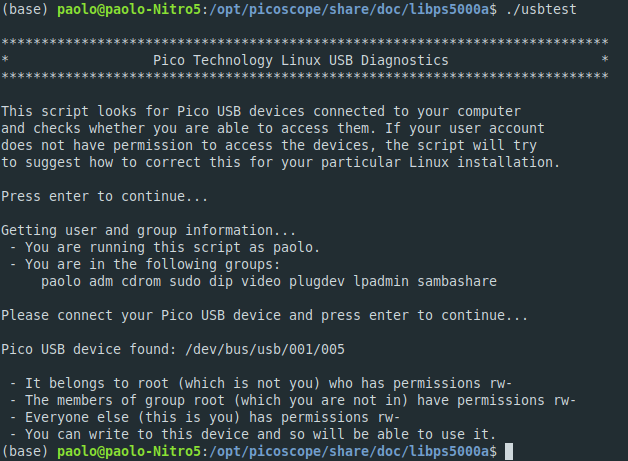
\includegraphics[scale=0.26]{Immagini/usbtest.png}
\end{figure}
Adesso che ci siamo assicurati che la libreria è installata correttamente, scarichiamo in una cartella apposita tutti i file d'esempio disponibili all'indirizzo github:
\begin{lstlisting}[language=bash]
git clone https://github.com/picotech/picosdk-c-examples
\end{lstlisting}
Una volta scaricato, andate nella cartella:
\begin{lstlisting}[language=bash]
cd ps5000a/linux-build-files/
\end{lstlisting}
Dove "ps5000a" è la libreria che utilizzeremo per la nostra versione del Picoscope (5444D). Una volta in questa cartella copiate il file che si trova nella cartella "ps5000aCon":
\begin{lstlisting}[language=bash]
cp ../ps5000aCon/ps5000aCon.c .
\end{lstlisting}
e usate il seguente comando:
\begin{lstlisting}[language=bash]
./autogen.sh
\end{lstlisting}
Adesso è possibile incorrere in una serie di errori, di cui elenco le soluzioni:
\begin{enumerate}
\item \begin{lstlisting}[language=bash]
Can't exec "aclocal": No such file or directory at /usr/share/autoconf/Autom4te/FileUtils.pm line 326.
autoreconf: failed to run aclocal: No such file or directory
\end{lstlisting}
Soluzione:
\begin{lstlisting}[language=bash]
sudo apt-get install automake
\end{lstlisting}

\item \begin{lstlisting}[language=bash]
configure: error: libps5000a-1.1/ps5000aApi.h missing!
\end{lstlisting}
Soluzione:
Bisogna rimuovere dai seguenti file presenti nella attuale cartella: \verb|configure.ac| e \verb|ps5000aCon.c| tutti i riferimenti alle librerie \verb|libps5000a-1.1| in questo modo:\\
\verb|libps5000a-1.1|$\to$\verb|libps5000a| oppure \verb|...-1.1|$\to$\verb|...|
\end{enumerate}
Una volta risolti gli eventuali errori eseguire il seguente comando:
\begin{lstlisting}[language=bash]
make
\end{lstlisting}
Se appare questo output sul terminale:
\begin{lstlisting}[language=bash]
make  all-am
make[1]: Entering directory '/home/md13/Desktop/Fermilab/Magnetometer/INO/picosdk_C/ps5000a/linux-build-files'
CC       ps5000aCon.o
CCLD     ps5000aCon
make[1]: Leaving directory '/home/md13/Desktop/Fermilab/Magnetometer/INO/picosdk_C/ps5000a/linux-build-files'
\end{lstlisting}
Allora tutto ok! Dovrebbe essere presente adesso nella cartella un eseguibile che è possibile lanciare con il comando:
\begin{lstlisting}[language=bash]
./ps5000aCon
\end{lstlisting}


\section{Utilizzare il codice}
\subsection{Scaricare il codice aggiornato}
Ora all'indirizzo github: \url{https://github.com/paololeo-gm2/Picoscope}, è possibile trovare il codice di esempio modificato da me, per ottimizzare la presa dati con il Picoscope 5444D.
Adesso si può procedere in 2 modi:
\begin{enumerate}
\item Potete scaricare direttamente dalla cartella \textbf{code}, il file \textbf{ps5000aCon.c}, e sostituirlo all'attuale file presente nella cartella \textbf{linux-build-files} che avete scaricato nella sezione precedente.
\item Potete scaricare l'intero contenuto della repository di Github in una nuova cartella del vostro pc, con il comando:
\begin{lstlisting}
git clone https://github.com/paololeo-gm2/Picoscope
\end{lstlisting}
E successivamente ripetere i passaggi del capitolo precedente.
\end{enumerate}
Scelta la prima o la seconda opzione, una volta che avrete il file \textbf{ps5000aCon.c} a vostra dispozione, eseguite il comando
\begin{lstlisting}
make
\end{lstlisting}
Che vi creerà un eseguibile (\textbf{ps5000aCon}) che potrete eseguire con il comando:
\begin{lstlisting}
./ps5000aCon
\end{lstlisting}
\subsection{Menù del codice}
Una volta fatto partire il programma, questo cercherà di trovare il dispositivo che dovrà essere collegato al vostro pc tramite una porta USB e alimentato per potergli permettere di leggere tutti i 4 canali disponibili.\\
\noindent \textbf{NOTA: Se il vostro dispositivo è già aperto in un altra applicazione del vostro computer, allora non verrà trovato dal programma che state utilizzando, e viceversa.}\\
\noindent Se il dispositivo viene trovato, allora elencherà una serie di informazioni generali sul dispositivo di ingresso, le impostazioni di default dei 4 canali e un menù da dove è possibile cambiare il settaggio dei canali, dell'acquisione generale e dove sarà possibile far partire l'acquisizione:
\begin{tcolorbox}
\begin{Verbatim}[tabsize = 4]
Please select operation:

										C - Coupling AC/DC (Default = AC)
W - Triggered streaming				 V - Set voltages
R - Collect set of rapid captures	   I - Set timebase 
										A - ADC Counts/mV
										D - Set resolution
X - Exit
\end{Verbatim}
\end{tcolorbox}
\noindent Il menù, come si vede, è diviso in varie opzioni, tra cui quelle a \textbf{sinistra} sono dedicate a far partire l'acquisizione, mentra quelle a \textbf{destra} servono per cambiar le impostazioni dei canali.\\
\noindent Vediamo a cosa serve ogni opzione:
\begin{itemize}
\item \textbf{C - Coupling AC/DC (Default = AC)}\\
Questa opzione permette di cambiare l'accopiamento di ciascuno dei canali disponibili per il Picoscope, che di default sono impostati su AC. Sul terminale compare in output:
\begin{tcolorbox}
\begin{Verbatim}[tabsize = 4]
0 -> AC COUPLING
1 -> DC COUPLING
Specify coupling (0 or 1)
99 - switches channel off

Channel A:
\end{Verbatim}
\end{tcolorbox}
Dove come si vede è possibile anche spegnere uno qualunque dei canali, con l'opzione \textbf{99}.
\item \textbf{V - Set voltages}\\
Questa opzione permette di cambiare il fondo scala di ciascuno dei canali, che di default sono impostati a 5V (come scritto nelle informazioni generali che compaiono una volta che il dispositivo viene aperto dal programma). Sul terminale compare in output:
\begin{tcolorbox}
\begin{Verbatim}[tabsize = 4]
0 -> 10 mV
1 -> 20 mV
2 -> 50 mV
3 -> 100 mV
4 -> 200 mV
5 -> 500 mV
6 -> 1000 mV
7 -> 2000 mV
8 -> 5000 mV
9 -> 10000 mV
10 -> 20000 mV
Specify voltage range (0..10)
99 - switches channel off

Channel A:
\end{Verbatim}
\end{tcolorbox}
Anche in questo caso è possibile spegnere uno dei canali dell'oscilloscopio.\\
\noindent \textbf{NOTA}: Conviene spegnere i canali inutilizzati, perchè ciò permette, come vedremo, all'oscilloscopio di acquisire con una risoluzione più alta.
\item \textbf{I - Set timebase}\\
Questa opzione permette di settare il rate di campionamento, o più precisamente, di settare l'intervallo temporale di campionamento fra $samples$ consecutivi. Sul terminale compare in output:
\begin{tcolorbox}
\begin{Verbatim}[tabsize = 4]
Shortest timebase index available ... (... seconds).
Specify desired timebase: ...
Timebase used ... = ... sample interval
\end{Verbatim}
\end{tcolorbox}
Dove l'indice del $timebase$ più piccolo possibile, dipende dalla risoluzione impostata.\\
Per avere un'idea di quale indice utilizzare, conviene dare un'occhiata alle seguenti tabelle:
\begin{figure}[h!]
\centering
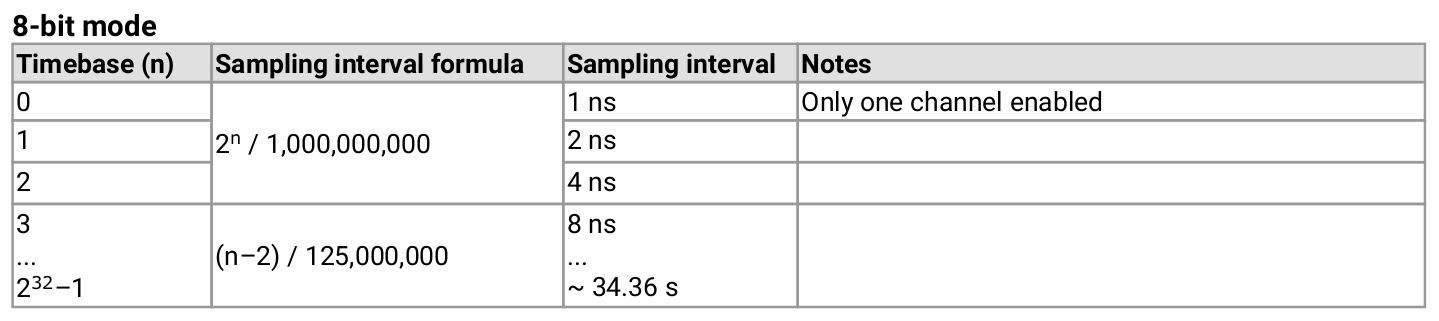
\includegraphics[scale=0.3]{Immagini/8_time.png}
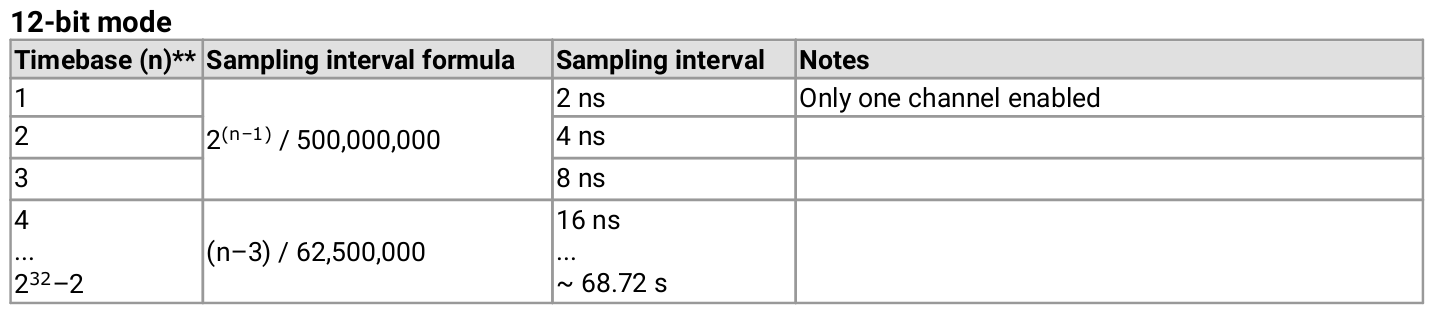
\includegraphics[scale=0.3]{Immagini/12_time.png}
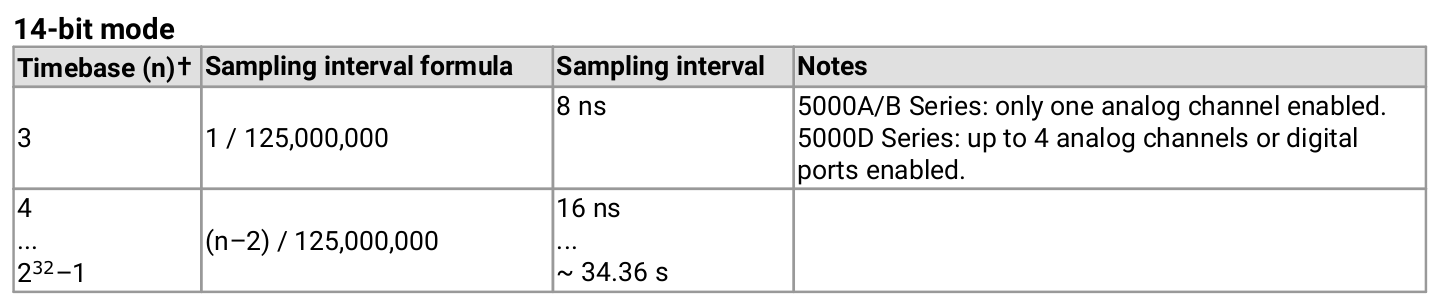
\includegraphics[scale=0.3]{Immagini/14_time.png}
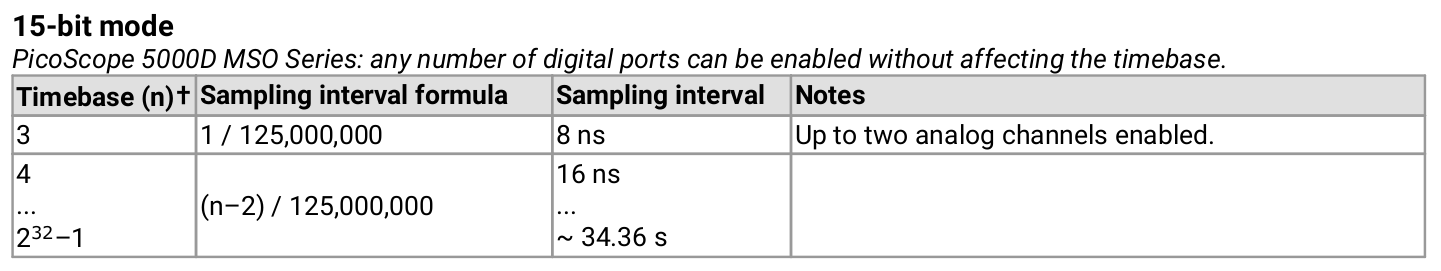
\includegraphics[scale=0.3]{Immagini/15_time.png}
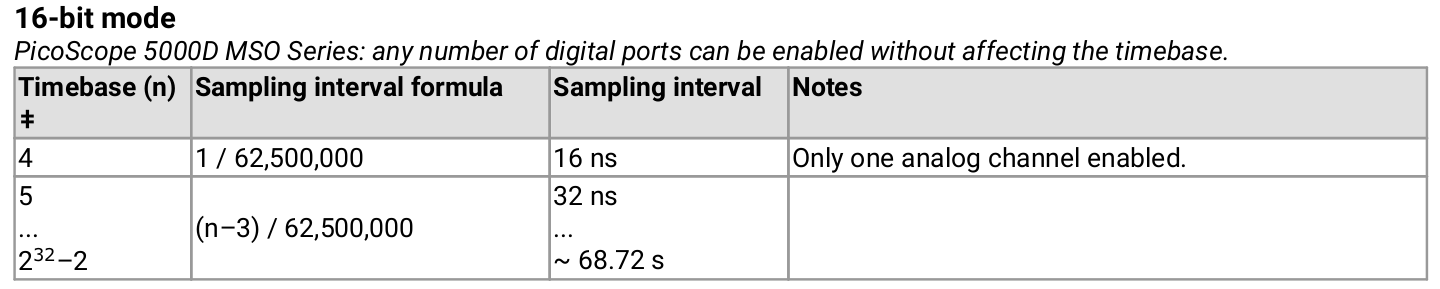
\includegraphics[scale=0.3]{Immagini/16_time.png}
\end{figure}
\item \textbf{A - ADC Counts/mV}\\
Questa opzione permette di cambiare l'unità di misura dei dati che vengono acquisiti da mV a ADC, e viceversa. Di default i dati vengono registrati in mV, per cui conviene non utilizzare questa funzione.
\item \textbf{D - Set resolution}\\
Questa opzione permette di settare la risoluzione del fondo scala selezionato per ogni canale, e avrà delle limitazioni in base al numero di canali attivi dell'oscilloscopio. Sul terminale compare in output:
\begin{tcolorbox}
\begin{Verbatim}[tabsize = 4]
Select device resolution:
0: 8 bits
1: 12 bits
2: 14 bits
3: 15 bits
4: 16 bits

Resolution [0..4]:
\end{Verbatim}
\end{tcolorbox}
Dove alcune delle opzioni potrebbe mancare, in base al numero di canali attivi.
\end{itemize}
Andiamo a vedere la modalità di acquisizione nel prossimo paragrafo.
\subsection{Modalità di acquisizione}
Rimane da vedere come funziona la modalità di acquisizione, prodotta dall funzione disponibile nel menù:
\textbf{R - Collect set of rapid captures} \\
\noindent Questà modalità permette di raccogliere un numero a piacere di forme d'onda, su ognuna delle queli può essere fissato un trigger che ne decide lo $start$ dell'acquisizione, con un numero a scelta di punti al suo interno (sia prima che dopo il segnale del trigger).\\
\noindent Se si seleziona questa modalità, in output sul terminale compare:
\begin{tcolorbox}
\begin{Verbatim}[tabsize = 4]
ACTUAL OPTIONS FOR BLOCK DATA CAPTURE (DATA STRUCTURE)

Number of waveforms = 1000
Number of Points per waveform = 2000
Number of Points pre-trigger = 500
Number of Points post-trigger = 1500

ACTUAL OPTIONS FOR BLOCK DATA CAPTURE (TRIGGER OPTIONS)

Trigger Channel = EXT
Trigger Voltage = 500 mV

Please select operation:

W - Set Number of Waveforms			 P - Set Number of Points per waveform
F - Set Number of Points pre-trigger	L - Set Number of points post-trigger

C - Set Trigger channel 		        V - Set Trigger Voltage

S - Continue
Operation:
\end{Verbatim}
\end{tcolorbox}
Dove vengono mostrate tutte le impostazioni di default della modalità di acquisizione (struttura dati e trigger), ed alcuni operazioni, dove è possibile cambiare una qualunque di queste impostazioni.\\
\noindent Le elenchiamo tutte in maniera rapida:
\begin{itemize}
\item \textbf{W - Set Number of Waveforms}\\
Setta il numero di forme d'onda che si vuole raccogliere.
\item \textbf{P - Set number of Points per waveforms}\\
Setta il numero di punti che possiede ogni forma d'onda. Se viene selezionata questa opzione, dopo il programma chiederà quanti punti pre-trigger si intende raccogliere (i punti post-trigger verrano automaticamente impostati come la differenza di questi due).
\item \textbf{F - Set Number of Points pre-trigger}\\
Setta il numero di punti che si intende raccogliere prima del segnale del trigger (questo numero deve necessariamente essere minore del numero di punti totale per forma d'onda). Se si seleziona questa opzione, il numero di punti post-trigger viene automaticamente settato come la differenza fra il numero di punti totale e il numero di punti pre-trigger appena selezionato.
\item \textbf{L - Set Number of Points post-trigger}\\
Setta il numero di punti che si intende raccogliere dopo il segnale del trigger (questo numero deve necessariamente essere minore del numero di punti totale per forma d'onda). Se si seleziona questa opzione, il numero di punti pre-trigger viene automaticamente settato come la differenza fra il numero di punti totale e il numero di punti post-trigger appena selezionato.
\item \textbf{C - Set Trigger channel}\\
Setta il canale sul quale agisce il trigger (il quale deve essere necessariamente abilitato). In output al terminale compare una finestra simile a questa:
\begin{tcolorbox}
\begin{Verbatim}[tabsize = 4]
0 -> A
1 -> B
2 -> C
3 -> D
4 -> EXT

Trigger Channel:
\end{Verbatim}
\end{tcolorbox}
\item \textbf{V - Set Trigger Voltage}\\
Setta il valore della tensione che il segnale del canale selezionato del trigger deve superare affinchè scatti il segnale del trigger (il quale si consiglia di non superare i 5V). In output al terminale compare una finestra simile a questa:
\begin{tcolorbox}
\begin{Verbatim}[tabsize = 4]
Trigger Voltage:
\end{Verbatim}
\end{tcolorbox}
\item \textbf{S - Continue}\\
Questa opzione fa partire l'acquisizione con le impostazioni elencate sopra.
\end{itemize}

\noindent Una volta fatta partire l'acquisizione, il programma salva i dati raccolti in un file nella cartella col nome \textbf{block.txt}, il quale avrà una struttura di questo tipo:
\begin{tcolorbox}
\begin{Verbatim}[tabsize = 4]
Time(ns)		ADC_ChA		mV_chA		ADC_chB		mV_chB
...			...			...			...			...
...			...			...			...			...
...			...			...			...			...
\end{Verbatim}
\end{tcolorbox}

Il quale dovrà poi essere analizzato a parte, e opportunamente salvato con un nome diverso.
 
\end{document}
